\documentclass[10pt]{beamer}

\usepackage{bm}
\usepackage{simplewick}
\usetheme{Berkeley}
\usepackage{multicol}
\usepackage{hyperref}
\usepackage{slashed}
\usepackage{graphicx}


\usecolortheme{lily}
\begin{document}
	\title{Extra Dimensions \& Gravitons \\ FYS4560}
	\author{\fontfamily{Decadence}\selectfont Sean B.S. Miller}
	\institute{\fontfamily{Decadence}\selectfont University of Oslo}
	\maketitle
	
	
	\begin{frame}
		\frametitle{Introduction}
		There are 3 different types of spatial extra dimensions (ED) models.
		\begin{itemize}
			\item \emph{Large}
			\item \emph{Warped}
			\item \emph{Universal}
		\end{itemize}
		
		Arkani-Hamed, Dimopoulos, and Dvali (1998) propsed the ADD-model\footnote{arXiv: hep-ph/9803315} (large ED)\\
		Randall and Sundrum (1999) proposed RS1-model\footnote{arXiv: hep-ph/9905221} (warped ED)\\
	\end{frame}
	
	\begin{frame}
		\frametitle{Kaluza-Klein theory}
		From linearised gravity,
		
		\begin{equation}
			g_{\mu\nu} = \eta_{\mu\nu} + h_{\mu\nu},
		\end{equation}
		
		we can find an interaction term $h_{\mu\nu}T^{\mu\nu}$ and a kinetic term for $h_{\mu\nu}$ in the Lagrangian density. However, a mass term for $h_{\mu\nu}$ can be suggested as
		
		\begin{equation}
			ah_{\mu\nu}h^{\mu\nu} + b(\eta_{\mu\nu}h^{\mu\nu})^2
		\end{equation}
		
		Markus Fierz and Wolfgang Pauli (1939) showed\cite{FP} that $a=-b$ in order to avoid unphysical results. The result of this was the Fierz-Pauli Lagrangian for massive gravity.
		
	\end{frame}
	
	\begin{frame}
		\frametitle{Kaluza-Klein theory}
		Kaluza assumed the metric could be written:
		
		\begin{equation}
			\hat{h}_{ab} = 
			V_d^{-1/2}\begin{pmatrix}
			h_{\mu\nu} + \eta_{\mu\nu}\phi & A_{\mu i}\\
			A_{\nu j} & 2\phi_{ij}
			\end{pmatrix}
		\end{equation}
		
		Kaluza assumed that these fields could be written as expansions, i.e.
		
		\begin{equation}
			h_{\mu\nu}(x,y) = \sum_{\substack{n=\{n_1,n_2,\ldots,n_5\}; \\ n_i\in\mathbb{Z}\:\forall\:i}} h_{n,\mu\nu}(x)Y_n(y)
		\end{equation}
		
		and similarly for $A_{\mu i}$ and $\phi$. The modes have to satisfy the Fierz-Pauli equations of motion. These, when combined, will show that $h_{\mu\nu}$ satisfies:
		
		\begin{equation}
			(\Box + m_n^2)(h_{n,\mu\nu}-\frac{1}{2}\eta_{\mu\nu}h_{n,\sigma}^\sigma) = 0 
		\end{equation}
		
		where $m_n^2 = \frac{4\pi^2 n^2}{R^2}$.
	\end{frame}
	
	\begin{frame}
		\frametitle{Kaluza-Klein theory}
		Through some non-trivial steps, one can find a Lagrangian with mass eigenstates $\tilde{h}_{n,\mu\nu}$, $\tilde{A}_{n,\mu i}$, and $\tilde{\phi}_{n,ij}$, defined from the previous fields.\\
		
		From the Hilbert-Einstein action:
		
		\begin{equation}
			S_d = \int d^4x \sqrt{-\hat{g}}\mathcal{L}(\hat{g},S,V,F)
		\end{equation}
		
		where $\hat{g}_{\mu\nu} = \eta_{\mu\nu} + \kappa(h_{\mu\nu} + \eta_{\mu\nu}\phi_{ii})$, we can find Feynman rules:
		
		\begin{equation}
			G_n^{\mu\nu\rho\sigma} = i\frac{\eta^{\mu\rho}\eta^{\nu\sigma} + \eta^{\mu\sigma}\eta^{\nu\rho} - \frac{2}{3}\eta^{\mu\nu}\eta^{\rho\sigma}}{k_G^2 - m_n^2 + i\epsilon}
		\end{equation}
		\begin{equation}
			-\frac{i\kappa}{8}\left[\gamma_\mu(k_1 + k_2)_ \nu + \gamma_\nu(k_1+k_2)_\mu - 2\eta_{\mu\nu}(\slashed k_1 + \slashed k_2 - 2m_f)\right]
		\end{equation}
		
	\end{frame}
	
	\begin{frame}
		\frametitle{ADD-model}
		The ADD model is mainly based on 3 features:
		
		\begin{itemize}
			\item There exists $d$ new spatial compact dimensions, with compactification volume $V_d$.
			\item The Planck scale is very low, at the order of one TeV,
			\item The SM degrees of freedom are localized on a 3D-brane, stretching along 3 non-compact spatial dimensions (i.e. the SM particles move in normal spacetime, not in the new dimension(s)).
		\end{itemize}
		
		The main idea is that $\bar{M} \sim 1\text{TeV}$.
		By demanding $S_4=S_{4+d}$, one finds the reduction formula:
		
		\begin{equation}
			M_{Pl}^2 = V_d \bar{M}^{d+2} \sim R^d \bar{M}^{d+2}
		\end{equation}
	\end{frame}
	
	\begin{frame}
		\frametitle{ADD-model}
		With $M_{Pl} \approx 1.22\times 10^{16}\:\text{TeV}$, one finds:
		
		\begin{align*}
		&d=1\quad\rightarrow\quad R\sim 10^{11}\:\text{m}\\
		&d=2\quad\rightarrow\quad R\sim 0.1\:\text{mm}\\
		&d=3\quad\rightarrow\quad R\sim 10^{-7}\:\text{mm}\\
		&\ldots\\
		&d=6\quad\rightarrow\quad R\sim 10^{-11}\:\text{mm}
		\end{align*}
		
		But Newton's law of gravity must still hold for $r>>R$.
	\end{frame}
	
	\begin{frame}
		\frametitle{RS1-Model}
		RS1-model is quite different. They assumed space had $S^1/\mathbb{Z}^2$ "orbifold" structure. At two points there existed a 3-brane:
		
		\begin{figure}[H]
			\centering
			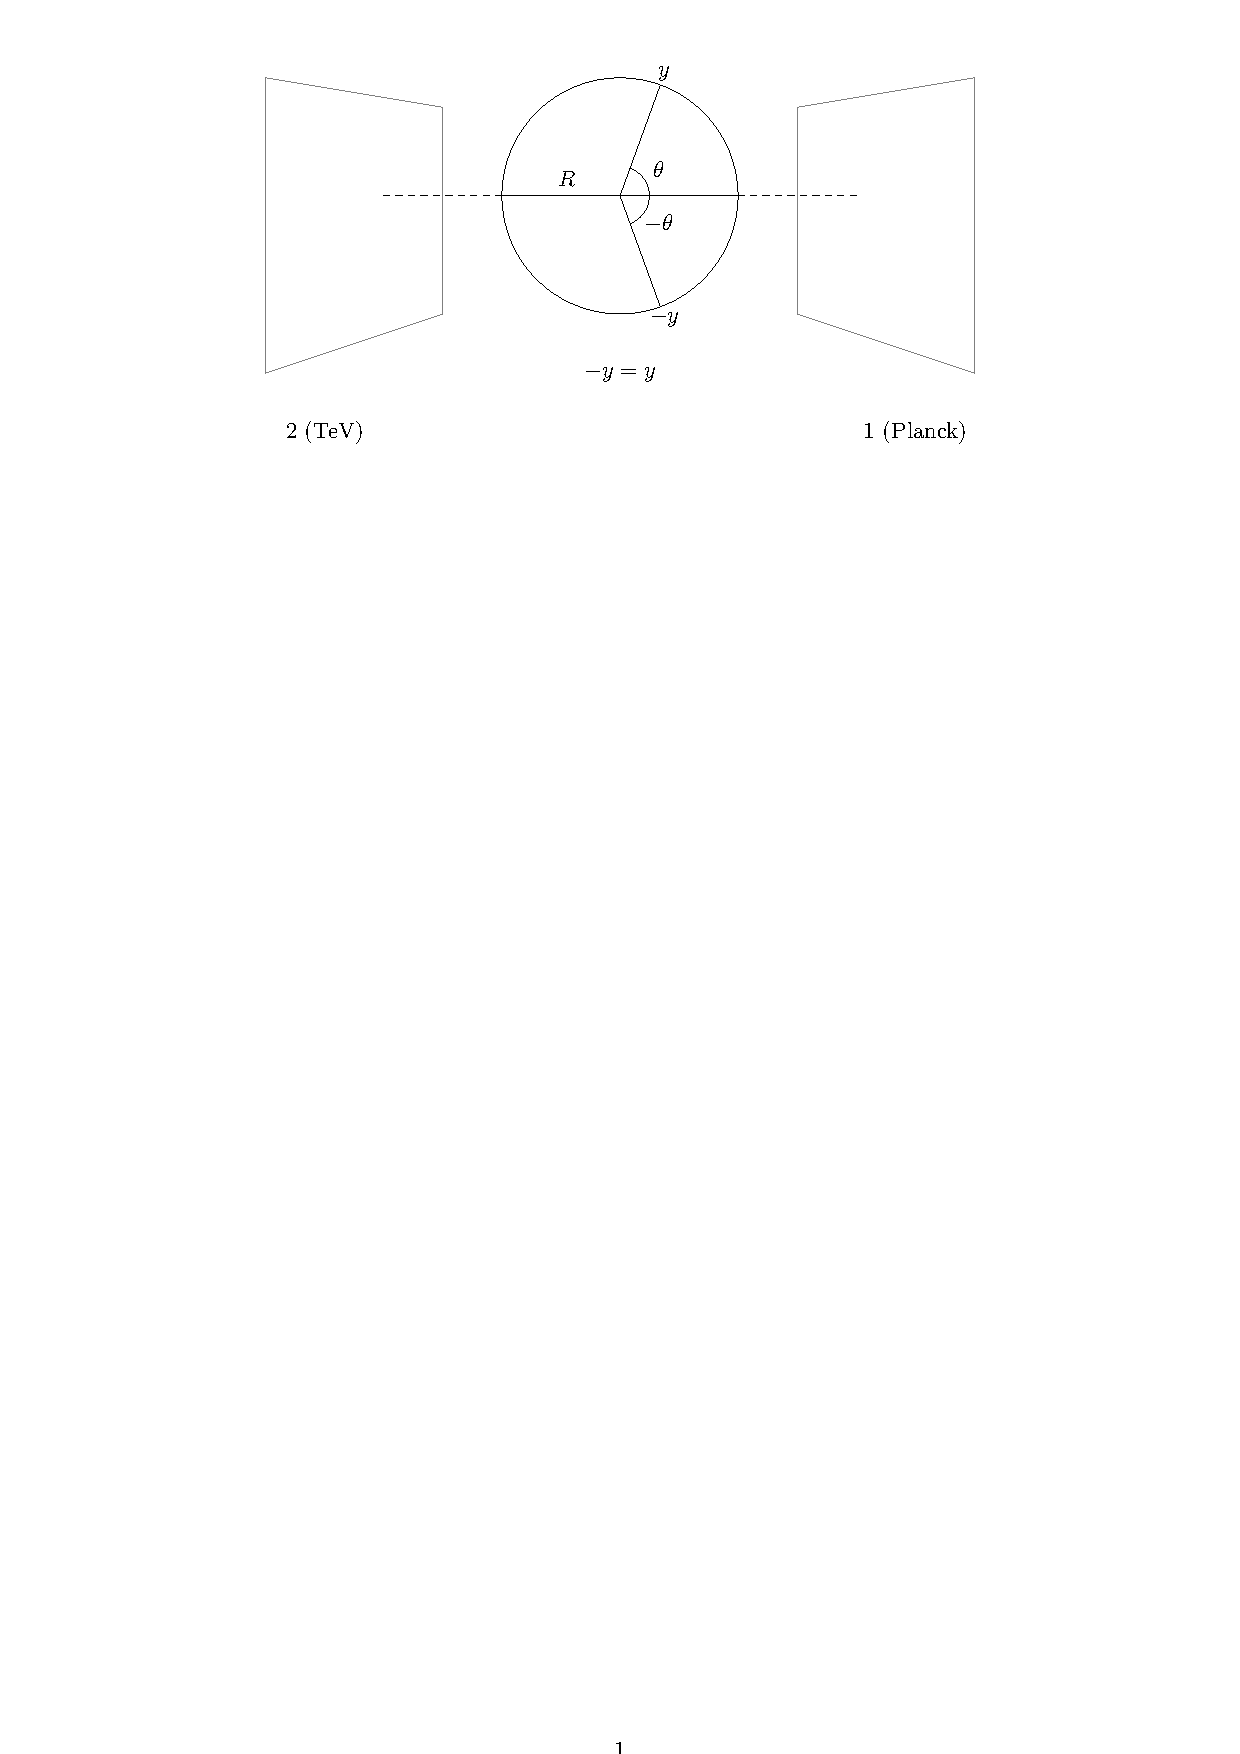
\includegraphics[trim={12cm 22cm 11.5cm 0cm},scale=0.4]{RS1.pdf}
			\label{fig:gravitonChannel}
		\end{figure}
		
		From Poincare invariance, it was found:
		
		\begin{equation}
			ds^2 = e^{-2A(y)}\eta_{\mu\nu}dx^\mu dx^\nu + dy^2
		\end{equation}
		
		Due to $\mathbb{Z}^2$-symmetry, have $A(y) = A(-y) = A(|y|)$. Solving the Einstein equations let Randall and Sundrum find $A(y) = k|y|$, $k=\sqrt{\frac{-\Lambda}{24M^3}}$.
		
	\end{frame}
	
	\begin{frame}
		\frametitle{RS1-Model}
		The metric forces a new reduction formula:
		\begin{equation}
			M_{Pl}^2 = \frac{M_5^3}{k}\left[1-e^{-2kR\pi}\right]
		\end{equation}
		For $M_5$ to solve the hierarchy problem, one has to require $kR \sim 12 \rightarrow e^{k\pi R} \sim 10^{15}$.\\
		
		With a new metric form, one has to repeat the KK mode expansion:
		
		\begin{equation}
			h_{\mu\nu}(x,\theta) = \sum_{n=0}^\infty h_{\mu\nu}^{(n)}(x)\frac{\chi_n(\theta)}{R}
		\end{equation}
		
		where $\chi_0(y) = 2\sqrt{kR}e^{-2kR|\theta|}$, and
		
		\begin{equation}
			\chi_n(y) = N_n\left[ C_1Y_2\left(\frac{m_n}{k}e^{kR|\theta|}\right) +   C_2J_2\left(\frac{m_n}{k}e^{kR|\theta|}\right)\right] \quad,\quad n\neq 0
		\end{equation}
	\end{frame}
	
	\begin{frame}
		\frametitle{RS1-model}
		On TeV brane, KK mode masses are
		\begin{equation}
			m_n = \beta_n ke^{-kR\pi}, \quad J_1(\beta_n) = 0\:\forall\: n\in\mathbb{N}
		\end{equation}
		
		Unlike the ADD-model, the masses are clearly separated. This means the sum over the KK tower is not necessary.\\
		Comparing RS1 Hilbert-Einstein action with the general KK action, one will see that:
		
		\begin{equation}
			\kappa = \sqrt{2}\frac{\beta_1}{m_1}\frac{k}{M_{Pl}}
		\end{equation}
		
		meaning RS1 is completely determined by two constants.
	\end{frame}
	
	\begin{frame}
		\frametitle{Proton-proton collisions}
		One channel for measuring the models is through the $pp\rightarrow G\rightarrow l^+l^-$ ($q\bar{q}\rightarrow G\rightarrow l^+l^-$):
		
		\begin{figure}[H]
			\centering
			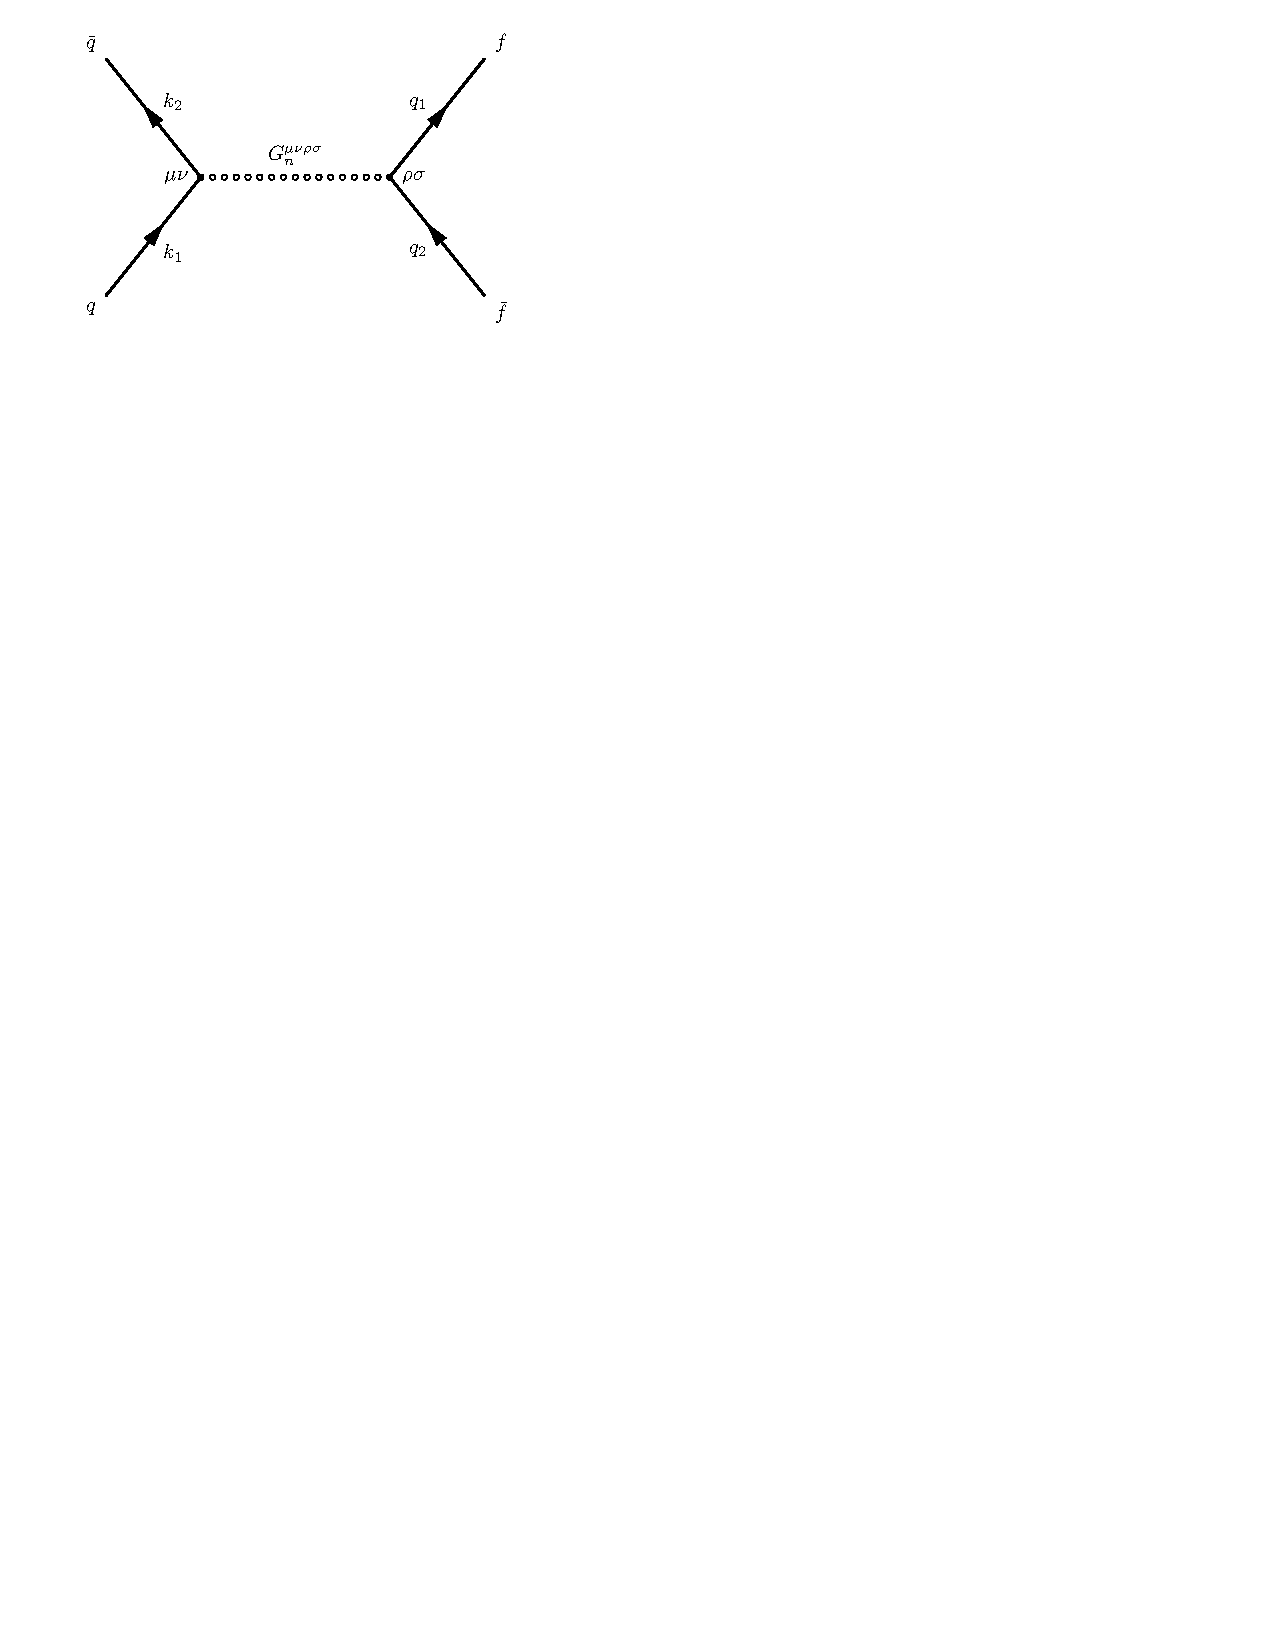
\includegraphics[trim={0.5cm 22cm 11.5cm 0cm},scale=0.5]{../feynGraphs/qqbar_G_ffbar}
		\end{figure}
		
	\end{frame}
	
	\begin{frame}
		\frametitle{Proton-proton collisions}
		After a little math...
	\end{frame}
	
	\begin{frame}
		\frametitle{Proton-proton collisions}
		\begin{equation}
		\frac{d\sigma_{G}}{d\cos(\theta)} = \frac{1}{2}\pi Q_f^2s^6|C_4|^2\left[1-3\cos^2(\theta) + 4\cos^4(\theta)\right]
		\end{equation}
		
		where $C_4 = \frac{\kappa^2}{8\pi} D(s)$ and $D(s) \equiv \sum_{n} \frac{1}{k_G^2 - m_n^2 + i\epsilon}$.
		
		\begin{figure}[H]
			\centering
			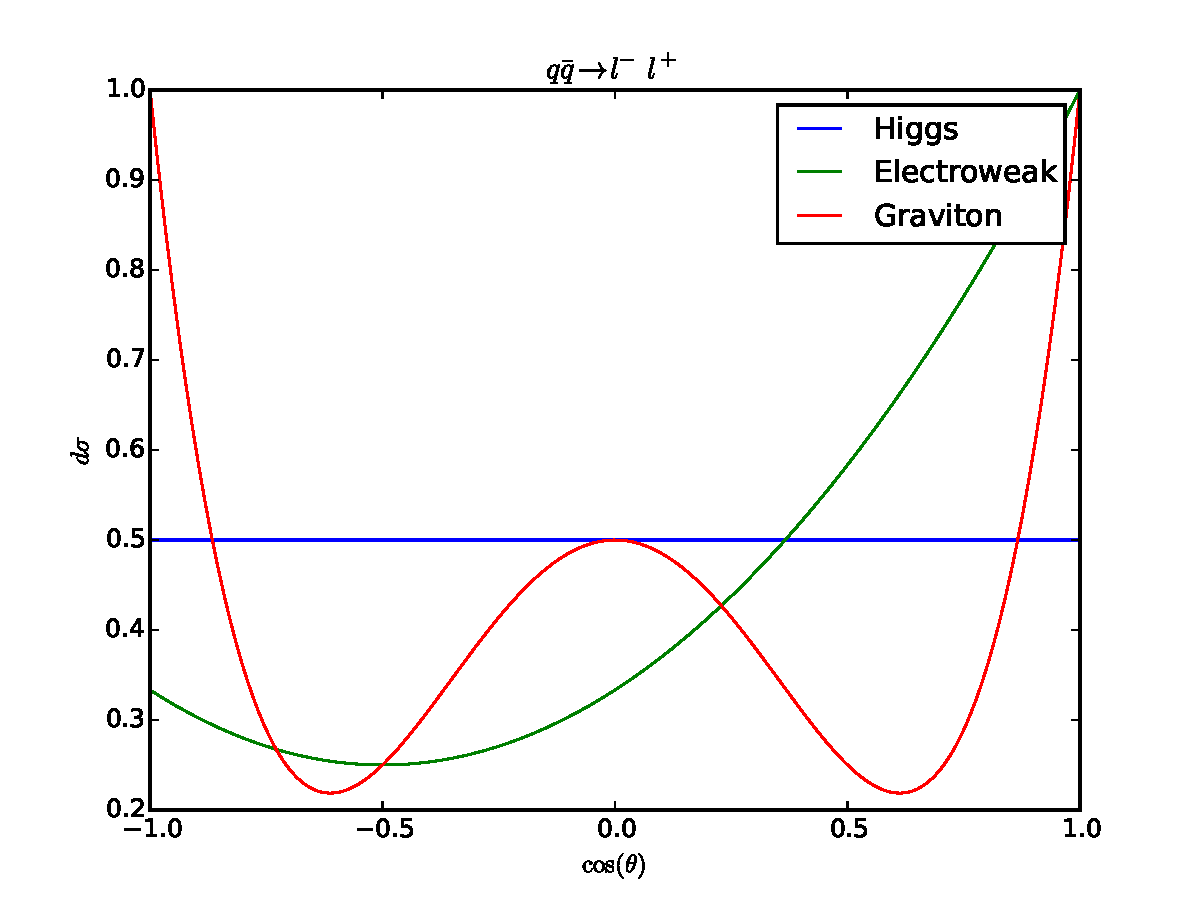
\includegraphics[scale=0.2]{../angDist.pdf}
		\end{figure}
		
	\end{frame}
	
	\begin{frame}
		\frametitle{Gravitons at the LHC}
		\begin{figure}[H]
			\centering
			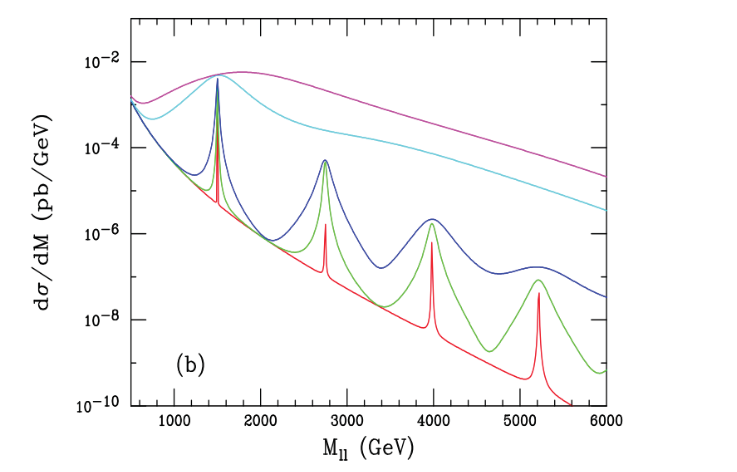
\includegraphics[scale=0.3]{cs.png}
		\end{figure}
	\end{frame}
	
	\begin{frame}
		\frametitle{Conclusions}
	\end{frame}
	
	\begin{frame}
		\frametitle{References}
		\begin{thebibliography}{9}
			\bibitem{Dvergsnes}
			E.W. Dvergsnes, \href{http://bora.uib.no/bitstream/handle/1956/847/THESIS.pdf?sequence=1}{"\emph{Extra Dimensions at Particle Colliders}"}, 2004, UiB
			\bibitem{HLZ}
			T. Han, J.D. Lykken, and R.-J. Zhang,
			\href{http://journals.aps.org/prd/abstract/10.1103/PhysRevD.59.105006}{\emph{Phys. Rev.} {\bfseries D 59} (1999) 105006}, doi:10.1103/PhysRevD.59.105006 \href{http://xxx.lanl.gov/abs/hep-ph/9811350v4}{hep-ph/9811350v4}
			\bibitem{AOPW}
			B.C. Allanach, K. Odagiri, M.A. Parker, and B.R. Webber,
			\href{http://iopscience.iop.org/article/10.1088/1126-6708/2000/09/019/meta;jsessionid=8B906F8B155A00E75050CBB02B18326C.c4.iopscience.cld.iop.org}{JHEP 0009:019,2000}, doi:10.1088/1126-6708/2000/09/019, \href{http://arxiv.org/abs/hep-ph/0006114v2}{hep-ph/0006114v2}
			\bibitem{FP}
			M. Fierz, P. Wolfgang, \href{http://rspa.royalsocietypublishing.org/content/173/953/211}{Proc. Roy. Soc. Lond. A173: 211–232}, doi: 10.1098/rspa.1939.0140
			\bibitem{BKSV}
			E.E. Boos, Y.A. Kubyshin, M.N. Smolyakov, and I.P. Volobuev, NPI MSU 2001-21/661, \href{http://arxiv.org/abs/hep-th/0105304}{hep-th/0105304}
			\bibitem{DHR}
			H. Davoudiasl, J.L Hewett, and T. G. Rizzo, \href{http://journals.aps.org/prl/abstract/10.1103/PhysRevLett.84.2080}{Phys. Rev. Lett. $\bm{84}$ 3370 (1999)}, doi:10.1103/PhysRevLett.84.2080, \href{http://arxiv.org/pdf/hep-ph/9911262v2.pdf}{hep-ph/9911262v2}
			\bibitem{K}
			Y.A. Kubyshin, (2001), \href{http://arxiv.org/abs/hep-ph/0111027v2}{hep-ph/0111027v2}
		\end{thebibliography}
	\end{frame}

\end{document}